\PassOptionsToPackage{table}{xcolor}

\documentclass[a4,11pt]{aleph-notas-alpha}

%%--> Paquetes adicionales
\usepackage{enumitem}
\usepackage{textcomp}
\usepackage{multicol}
\usepackage{fvextra}
%%--> Preámbulo del material
%% --> Paquetes comunes
\usepackage{listings}
\usepackage{enumitem}
\usepackage{lipsum}
\usepackage{booktabs}
\usepackage{todonotes}
\usepackage[spanish,onelanguage,vlined,linesnumbered]{algorithm2e}
\setuptodonotes{color=colordef!40, size=\footnotesize}
\newcommand{\porhacer}[1]{\todo[inline]{\textbf{Por hacer:} #1}}

%% --> Definición de colores
\definecolor{codegreen}{HTML}{A5BE00}
\definecolor{codegray}{rgb}{0.5,0.5,0.5}
\definecolor{codepurple}{rgb}{0.58,0,0.82}
\definecolor{backcolour}{rgb}{0.95,0.95,0.92}

%% --> Estilo para código
\lstdefinestyle{mystyle}{
    language={[LaTeX]TeX}, % lenguaje
    basicstyle=\bfseries\ttfamily,
    keywordstyle=\color{colordef},
    commentstyle=\color{codegreen},
    inputencoding=utf8,
    showstringspaces=false,
    flexiblecolumns=true,
    stringstyle=\ttfamily\color{blue},
    extendedchars=true,
    emph={rm,bf,it,sf}, %...
    literate=%
    {ó}{{\'o}}1%
    {í}{{\'i}}1%
    {á}{{\'a}}1%
    {ú}{{\'u}}1%
}

%% --> Selección de estilo para el código
\lstset{
    style=mystyle,escapeinside={(*@}{@*)}
}

% Blancos tipográficos
\newcommand{\mq}{\hspace{0.5em}}  %medio cuadratín
\newcommand{\tq}{\hspace{0.33em}} % un terio de cuadratín
\newcommand{\qq}{\hspace{0.25em}} % un cuarto de cuadratín
\newcommand{\fs}{\hspace{0.125em}} % un octavo de cuadratín
\newcommand{\ep}{\hspace{0.05em}} % espacio de pelo

%% --> Nota para el material
\newcommand{\informacion}{\noindent{\small\color{colordef}
El presente material fue desarrollado por:

\begin{center}
\textbf{Daniel Lara}\\
\emph{Facultad de Ciencias, Escuela Politécnica Nacional}\\[2mm]


\textbf{Andrés Merino}\\
\emph{Facultad de Ciencias Exactas y Naturales, Pontificia Universidad Católica del Ecuador}
\end{center}

\medskip\noindent
La versión actual del material es 1.3-(Noviembre 2021). En caso de encontrar inconsistencias o errores en el presente material se pueden comunicar a \href{mailto:daniel.lara@alephsub0.org}{daniel.lara@alephsub0.org}. Para más información puedes visitar nuestro sitio web: \href{https://alephsub0.org}{alephsub0.org}. Si deseas colaborar con el desarrollo de este material, el código fuente está disponible en:   
\url{https://github.com/alephsub0/LaTeX_Guias.git}. Cualquier aporte (\emph{Pull request}) será de gran ayuda para mejorar este material. 

\medskip\noindent

\includegraphics[height=10pt]{Imagenes/CreativeCommos/cc.xlarge.png}

\includegraphics[height=10pt]{Imagenes/CreativeCommos/by.xlarge.png}

\includegraphics[height=10pt]{Imagenes/CreativeCommos/nc.xlarge.png}
Esta obra se encuentra bajo licencia Atribución-NoComercial-CompartirIgual 4.0 Internacional (CC BY-NC-SA 4.0) Para más información puede visitar: \url{https://creativecommons.org/licenses/by-nc-sa/4.0/}


%% -- > Aquí se incluyen los nombres de los colaboradores de estas guías:
% \medskip\noindent
% Otros colaboradores: Katheryn Yánes
}}

%%--> Formato para títulos
\titleformat{name=\section,numberless}[display]
  {\vspace*{-2mm}\bfseries\scshape\centering}
    {}{1ex}
    {\color{colortext}\large\titlerule\vspace{.05ex}
     }
    [\color{colortext}\vspace{.2ex}\titlerule]

\titleformat{\subsubsection}
    {\color{colortext}\normalsize\bfseries}
    {\thesubsubsection}{1em}{}
    
%% --> Datos de las guias
\universidad{Curso de \LaTeX}
\autor{Proyecto Alephsub0}
\materia{Introducción a \LaTeX}

%% --> Logos de las guias
\logouno[4.5cm]{Imagenes/Logos/LogoAlephsub0-02.png}
\longtitulo{0.6\linewidth}
\fecha{Noviembre de 2021}

%% --> Nuevos ambientes
% \definecolor{coloryt}{rgb}{0.769,0.188,0.169}
%% Ambientes
\makeatletter
%%  Keys temporales: |colorlat|
\def\tcb@@colorlat{colordef!50!black}
    \tcbset{ colorlat/.code = {\def\tcb@@colorlat{#1} } }
%%  Estilo de YouTube
\tcbset{ postitbeta/.style ={
    % -> Opciones generales
    breakable,enhanced,
    before skip=2mm,after skip=3mm,
    colback=\tcb@@color!50,colframe=\tcb@@color!20!black,
    boxrule=0.4pt,
    drop fuzzy shadow,
    left=6mm,right=2mm,top=0.5mm,bottom=0.5mm,
    sharp corners,rounded corners=southeast,arc is angular,arc=3mm,
    parbox=false,
    underlay unbroken and last = {%
        \path[fill=tcbcolback!80!black]
        ([yshift=3mm]interior.south east) --++ (-0.4,-0.1) --++ (0.1,-0.2);
        \path[draw=tcbcolframe,shorten <=-0.05mm,shorten >=-0.05mm]
        ([yshift=3mm]interior.south east) --++ (-0.4,-0.1) --++ (0.1,-0.2);
        \path[fill=\tcb@@colorlat,draw=none]
        (interior.south west) rectangle node[white]{\tcb@@icono} ([xshift=5.5mm]interior.north west);
        },
    underlay = {%
        \path[fill=\tcb@@colorlat,draw=none]
        (interior.south west) rectangle node[white]{\tcb@@icono} ([xshift=5.5mm]interior.north west);
        }
    }
    }
\makeatother

%% Recuadro para enlaces de YouTube
\definecolor{coloryt}{HTML}{ffcccc}
\newtcolorbox{tcbyoutube}
    {icono=\faYoutubePlay,color=coloryt,colorlat=red,postitbeta,colframe=red,leftright skip=1cm}
    
%% Comando para enlaces de YouTube
\newcommand{\YouTube}[4]%
    {
        \begin{tcbyoutube}
            \parbox{0.30\linewidth}{\href{#2}{\includegraphics[width=\linewidth]{#3}}}
            \hspace{2mm}
            \parbox{0.65\linewidth}{\footnotesize
            \textbf{#1}\\[1mm]
            \faLink\ \url{#2}\\[2mm]
            \scriptsize
            #4}
        \end{tcbyoutube}
    }
    
%% Recuadro para enlaces
\definecolor{coloren}{HTML}{B9F2BC}
\newtcolorbox{tcbenlace}
    {icono=\faLink,color=coloren,postit,leftright skip=1cm,fontupper=\small}

%% Recuadro para impresión
\definecolor{colorimp}{HTML}{F8F8FF}
\newtcolorbox{tcbimprimir}
    {icono=\faPrint,color=colorimp,postit,leftright skip=1cm,fontupper=\small}

%% Ambiente para código
\definecolor{colcod}{RGB}{174,218,255}
\newtcolorbox{tcbcodigo}
    {icono=\faCode,color=colcod,postit,top=-2mm,bottom=-2mm,leftright skip=1cm,fontupper=\small}

%% Ambiente para código LaTeX  
\usepackage{minted}
\usemintedstyle{borland}
\tcbuselibrary{minted}
\tcbset{listing engine=minted}
\newtcblisting{tcbLaTeX}{%
    icono=\faCode,color=colcod,postit,top=0mm,bottom=0mm,
    leftright skip=1cm,fontupper=\small,
    minted language=latex,minted style=colorful,
    listing only}
% \newtcolorbox{tcbcodigo}
%     {icono=\faCode,color=colcod,postit,top=-2mm,bottom=-2mm,leftright skip=1cm,fontupper=\small}

%% Ambiente para figuras 
\newtcolorbox[blend into=figures]{figura}[2][]
    {float=h,capture=hbox,title={#2},every float=\centering,
    arc=0mm,left=2mm,right=2mm,
    boxrule=0pt,
    colback=colordef!10,
    colbacktitle=colordef!80,fonttitle=\small,
    enhanced,attach boxed title to bottom,center title,
    #1}

%% Ambiente para tablas 
\newtcolorbox[blend into=tables]{tabla}[2][]
    {float=h,capture=hbox,title={#2},every float=\centering,
    arc=0mm,left=2mm,right=2mm,
    boxrule=0pt,
    colback=colordef!10,
    colbacktitle=colordef!80,fonttitle=\small,
    enhanced,center title,
    #1}

%% Ambiente para código LaTeX desplegado
\newtcblisting{tcbLaTeXb}{%
    icono=\faCode,color=colcod,postit,top=0mm,bottom=0mm,
    fontupper=\small,
    minted language=latex,minted style=colorful,listing side text}
\newtcblisting{tcbLaTeXs}{%
    icono=\faCode,color=colcod,postit,top=0mm,bottom=0mm,
    fontupper=\small,
    minted language=latex,minted style=colorful}

%% Recuadro para comando en línea
\DeclareTotalTCBox{\miverb}{ v }{
    fontupper=\ttfamily,nobeforeafter,tcbox raise base,arc=0pt,outer arc=0pt,
    top=0pt,bottom=0pt,left=0mm,right=0mm,
    leftrule=0pt,rightrule=0pt,toprule=0.3mm,bottomrule=0.3mm,boxsep=0.5mm,
    colback=colcod!10!white,colframe=colcod!50!black}{#1}


% -- Datos del libro
\nota{Guía 2}
\tema{Primeros pasos}
%%--> Opciones adicionales
\DontPrintSemicolon

%%%%%%%%%%%%%%%%%%%%%%%%%%%%%%%%%%%%%%%%
%%  Comienzo del documento
%%%%%%%%%%%%%%%%%%%%%%%%%%%%%%%%%%%%%%%%

\begin{document}

\encabezado

\informacion

\tableofcontents

\newpage
\vspace*{-18mm}


\begin{tabla}[label={tab:papersize}]{Tamaños de papel}
\rowcolors{2}{colordef!17}{colordef!10}
  \begin{tabular}{ccccccc}
    a0paper & a1paper & a2paper & a3paper & a4paper & a5paper & a6paper \\ b0paper & b1paper & b2paper & b3paper & b4paper & b5paper &  b6paper \\ c0paper & c1paper & c2paper & c3paper & c4paper & c5paper & c6paper \\ 
    b0j & b1j & b2j & b3j& b4j& b5j& b6j \\
    ansiapape & ansibpaper & ansicpaper & ansidpaper & ansiepaper & letterpaper & executivepaper \\  legalpaper 
  \end{tabular}
\end{tabla}

Por otra parte, los parámetros de medidas disponibles y más comunes son:

\begin{itemize}
    \item Ancho de texto (\texttt{textwidth})
    \item Altura de texto (\texttt{textheight})
    \item Margen superior (\texttt{top, tmargin})
    \item Margen inferior (\texttt{bottom, bmargin})
    \item Margen izquierdo (\texttt{left, lmargin, inner})
    \item Margen derecho (\texttt{right, rmargin, outer})
\end{itemize}

Existen opciones adicionales e información que puede ser consultada en la documentación del paquete, aunque un breve resumen se encuentra en la siguiente imagen:

\begin{figure}[H]
    \centering
    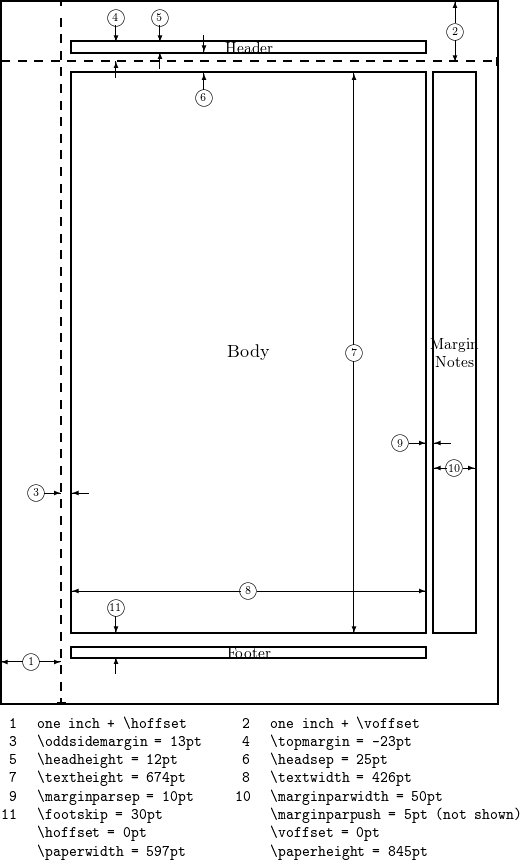
\includegraphics[width=0.75\textwidth]{Imagenes/Layout-dimensions.png}
\end{figure}

\newpage


El paquete babel es una de las «herramientas» básicas para la composición de textos pues permite modificar el idioma del documento; En algunos casos este paquete puede ser reemplazado por el siguiente código que modifica «manualmente» los parámetros que normalmente serían modificados por \texttt{babel}

\begin{tcbcodigo} \begin{lstlisting}
\renewcommand{\contentsname}{Contenido}
\renewcommand{\partname}{Parte}
\renewcommand{\appendixname}{Ap\'endice}
\renewcommand{\figurename}{Figura}
\renewcommand{\tablename}{Tabla}
\AtBeginDocument{\renewcommand\tablename{Tabla}}
\renewcommand{\abstractname}{Resumen}
\renewcommand{\refname}{Bibliograf\'{\i}a}
\end{lstlisting} \end{tcbcodigo}

\begin{advertencia}
En general, se recomienda usar los acentos con la forma \verb@\'@ en lugar del acento directo desde el teclado.
\end{advertencia}





El archivo que contiene el código fuente posee la extensión \texttt{.tex} mientras que el archivo que contiene los registros del proceso de compilación poseen la extensión  \texttt{.log}. Una tabla completa con los archivos más usuales en la compilación de un documento se encuentran a continuación:

\begin{tabla}[label={tab:2.1}]{Tipos de archivos usados en \TeX{} y \LaTeX{}}
    \centering
    \rowcolors{2}{colordef!17}{colordef!10}
    \begin{tabular}{ll}
        \toprule
        \textbf{Tipo de archivo} & \textbf{Extensiones más comunes}  \\ \midrule
        Código base &  \texttt{.tex} \\ 
        Base de datos para bibliografía & \texttt{.bib}\\
        Índice & \texttt{.ind}\\
        Imágenes & \texttt{.ps},\texttt{.eps},\texttt{.tif},\texttt{.png},\texttt{.jpg},\texttt{.gif},\texttt{.pdf}\\
        Clases  & \texttt{.cls}\\
        Paquetes & \texttt{.sty}\\
        Auxiliar & \texttt{.aux}\\
        Tabla de contenidos & \texttt{.toc}\\
        Lista de figuras\fs/\fs Tablas & \texttt{.lof},\texttt{.lot}\\
        Medidas del tipo & \texttt{.tfm}\\
        Transcripción & \texttt{.log}\\
        Índice alfabético & \texttt{.idx},\texttt{.ind}\\
        TrueType & \texttt{.ttf}\\
        OpenType & \texttt{.otf}\\
        \bottomrule
    \end{tabular}
\end{tabla}


Regresando a la estructura del archivo fuente tenemos lo siguiente: 
El primer comando especifica la \textit{clase} de documento que vamos a generar y tiene la siguiente estructura:

\begin{tcbcodigo} \begin{lstlisting}
\documentclass[Opciones del documento]{Tipo de documento}
\end{lstlisting} \end{tcbcodigo}

\noindent
Para el desarrollo de los ejemplos usaremos:

\begin{tcbcodigo} \begin{lstlisting}
\documentclass[10pt]{article}
\end{lstlisting} \end{tcbcodigo}

Un documento básico en \LaTeX{} se compone de dos partes: el \textit{preámbulo} y el \textit{cuerpo}. El preámbulo, incluye la \emph{clase}\footnote{Una clase es un archivo de extensión \texttt{.cls} que define el formato del documento.} del documento, paquetes a usar y configuraciones adicionales, mientras que el cuerpo contiene el texto y fórmulas matemática que van a ser mostradas.


\begin{tcbcodigo} \begin{lstlisting}
% Preambulo
\documentclass[10pt]{article}

\usepackage[utf8]{inputenc}
\usepackage[T1]{fontenc}
\usepackage[spanish]{babel}
\usepackage{geometry}

\begin{document}
% Cuerpo
Hola Mundo
\end{document}
\end{lstlisting} \end{tcbcodigo}

\section{Escritura de texto}

\subsection{Espacios}

\LaTeX \hspace{3pt} trata todos los caracteres en blanco, tales como el espacio en blanco o el tabulador, como un solo espacio. El espacio en blanco al principio de una linea se ignora, y un salto de linea aislado se trata como espacio en blanco. Una linea vacía entre dos lineas de texto define el fin de un párrafo. Varias lineas vacías se tratan igual que una sola linea vacía.


\subsubsection{Espacios Horizontal}

\LaTeX\hspace{1.5pt} determina los espacios entre palabras y oraciones automáticamente.  Para añadir espacio horizontal, se usa \verb|\hspace{|\emph{longitud}\verb|}|. Si el espacio debiera mantenerse incluso si cae al final o al principio de renglón, use \verb|\hspace*| en  lugar de \verb|\hspace|.
\noindent
La \emph{longitud} en el caso más simple es sólo un número más una unidad.  Las unidades más importantes se listan en el cuadro~\ref{units}.

\begin{tabla}[label={units}]{\TeX \hspace{1.5pt} Unidades.}
  \rowcolors{2}{colordef!17}{colordef!10}
  \begin{tabular}{@{}rl@{}}
    \toprule
    \textbf{Código} & \textbf{Descripción} \\ \midrule
    \texttt{mm}          & milímetro $\approx 1/25$~pulgada \\
    \texttt{cm}          & centímetro = 10~mm  \\
    \texttt{in}          & pulgada $=$ 25,4~mm \\
    \texttt{pt}          & punto $\approx 1/72$~pulgada $\approx \frac{1}{3}$~mm  \\
    \texttt{em}          & $\approx$ anchura de una `M' en la fundición actual \\
    \texttt{ex}          & $\approx$ altura de una `x' en la fundición actual \\
    \EscVerb{\\baselineskip} & altura de un salto de linea \\ \bottomrule
  \end{tabular}
\end{tabla}

\noindent
La orden \verb"\hfill" genera un espacio que se expande hasta llenar todo el espacio sobrante en un renglón o página.

\subsubsection{Espaciado Vertical}

El espacio entre párrafos, secciones, subsecciones,\ldots{}  lo determina automáticamente \LaTeX.  Si es necesario, un espacio vertical adicional \emph{entre dos párrafos} puede añadirse con la orden \verb|\vspace{|\emph{longitud}\verb|}|. Si el espacio debe preservarse en lo alto o en lo bajo de la página, use la versión  de la orden con asterisco, \verb|\vspace*|, en lugar de \verb|\vspace|. Espacio adicional entre dos lineas del \emph{mismo} párrafo o dentro de una tabla se indica con el comando \verb|\\[|\emph{longitud}\verb|]|

\subsubsection{Espacio duro}

En algunos casos se requiere colocar espacios pero estos no deben separarse en un salto de linea, estos se conocen como espacios duros o irrompibles pues de coincidir al final de una linea mueven todo el bloque de texto y no permiten que se separen. Para introducir este tipo de espacios usamos una virgulilla (\verb@~@).

\subsection{Caracteres especiales}

Los siguientes símbolos son caracteres reservados que tienen un significado especial en \LaTeX. Si los escribimos directamente, no se imprimirán, sino que obligarán a \LaTeX a hacer cosas que no se pretendía hacer.
 \begin{center}
  \verb.#  $  %  ^  &  _  {  }  ~  \ ". %$
 \end{center}

Se pueden usar algunos de estos caracteres añadiendo una barra invertida como prefijo:
 \begin{center}
  \verb.\# \$ \% \^{} \& \_ \{ \} \~{}.
 \end{center}
obteniendo así los símbolos: \# \$ \% \^{} \& \_ \{ \} \~{}.

Para la barra invertida se deberá escribir \verb@\backslash@. y la forma correcta de poner comillas es usar dos~\textasciigrave~(acentos graves) para abrirlas y dos~\textquotesingle~(apóstrofos) para cerraras.


\subsection{Alineación (\emph{flushleft}, \emph{flushright} y \emph{center})}

Los entornos \texttt{flushleft} y \texttt{flushright} generan párrafos alineados a la izquierda o a la derecha respectivamente. El entorno \texttt{center} genera texto centrado.

\subsection{Fundiciones y tamaños}

\LaTeX\hspace{1.5pt} escoge la fundición y el tamaño de fundición apropiados basándose en la estructura lógica del documento (secciones, notas al pie, \ldots).   Para cambiar fundiciones y tamaños se puede usar las órdenes listadas en los cuadros~\ref{fonts} y~\ref{sizes}. El cuadro~\ref{tab:pointsizes}
muestra los tamaños absolutos en puntos para estas órdenes según se implementan en las clases de documentos normales.

\begin{tabla}[label={fonts}]{Fundiciones}       
 \rowcolors{2}{colordef!17}{colordef!10}
  \begin{tabular}{@{}rl@{\qquad}rl@{}}
    \toprule
    \textbf{Código} & \textbf{Descripción} & \textbf{Código} & \textbf{Descripción} \\ \midrule
    \EscVerb{\\textrm{...}}        &      \textrm{{rematada}}&
    \EscVerb{\\textsf{...}}        &      \textsf{{palo seco}}\\
    \EscVerb{\\textmd{...}}        &      \textmd{peso medio}&
    \EscVerb{\\textbf{...}}        &      \textbf{{negrita}}\\
    \EscVerb{\\textup{...}}      &       \textup{{recta}}&
    \EscVerb{\\textit{...}}        &       \textit{{cursiva}}\\
    \EscVerb{\\textsl{...}}        &       \textsl{{oblicua}}&
    \EscVerb{\\textsc{...}}        &       \textsc{{Versalitas}}\\
    \EscVerb{\\emph{...}}          &            \emph{destacada} &
    \EscVerb{\\texttt{...}}        &      \texttt{de máquina}\\\bottomrule
  \end{tabular}
\end{tabla}

\begin{tabla}[label={sizes}]{Tamaños de fundición.}
\index{font size}
\rowcolors{2}{colordef!17}{colordef!10}
\begin{tabular}{@{}ll}
\toprule
\textbf{Código} & \textbf{Descripción} \\ \midrule
\EscVerb{\\tiny}      & \tiny        tiny\\
\EscVerb{\\scriptsize}   & \scriptsize  scriptsize\\
\EscVerb{\\footnotesize} & \footnotesize  footnotesize\\
\EscVerb{\\small}        &  \small          small\\
\EscVerb{\\normalsize}   &  \normalsize  normalsize \\
\EscVerb{\\large}        &  \large       large\\
\EscVerb{\\Large}        &  \Large       Large \\[5pt]
\EscVerb{\\LARGE}        &  \LARGE       LARGE \\[5pt]
\EscVerb{\\huge}         &  \huge        huge \\[5pt]
\EscVerb{\\Huge}         &  \Huge        Huge\\[5pt]\bottomrule
\end{tabular}
\end{tabla}

\begin{tabla}[label={tab:pointsizes}]{Tamaños absolutos en puntos para las clases normales.}
\rowcolors{2}{colordef!17}{colordef!10}
\begin{tabular}{lrrr}
\toprule
\multicolumn{1}{c}{\textbf{Tamaños}} &
\multicolumn{1}{c}{\textbf{10pt (por omisión) }} &
          \multicolumn{1}{c}{\textbf{opción 11pt}}  &
          \multicolumn{1}{c}{\textbf{opción 12pt}}\\ \midrule
\EscVerb{\\tiny}       & 5pt  & 6pt & 6pt\\
\EscVerb{\\scriptsize} & 7pt  & 8pt & 8pt\\
\EscVerb{\\footnotesize} & 8pt & 9pt & 10pt \\
\EscVerb{\\small}        & 9pt & 10pt & 11pt \\
\EscVerb{\\normalsize} & 10pt & 11pt & 12pt \\
\EscVerb{\\large}      & 12pt & 12pt & 14pt \\
\EscVerb{\\Large}      & 14pt & 14pt & 17pt \\
\EscVerb{\\LARGE}      & 17pt & 17pt & 20pt\\
\EscVerb{\\huge}       & 20pt & 20pt & 25pt\\
\EscVerb{\\Huge}       & 25pt & 25pt & 25pt\\\bottomrule
\end{tabular}
\end{tabla}

\section{Otros comandos}

A continuación se encuentra una pequeña lista de otros comandos útiles en el desarrollo de documentos:

\begin{itemize}
    \item \verb@\renewcommand{\baselinestretch}{1.5}@ Modificación del interlineado
    \item \verb@\pagestyle{empty}@ Eliminar numeración de página
    \item \verb@\parindent=0mm@ Eliminar las sangría
    \item \verb@\newpage@ Agrega una nueva página
    \item \verb@\pagebreak@ Inserta un salto de página
    \item \verb@\today@ Imprime la fecha actual
\end{itemize}


\subsection{Separación de palabras}

En general, con el paquete babel aseguramos que la mayoría de las palabras se separen correctamente. Sin embargo, es posible que algunas palabras no se separen correctamente, para subsanar este error podemos especificar la forma para separar las palabras de la siguiente manera:

\begin{tcbcodigo} \begin{lstlisting}
Electroence\-falografista
\end{lstlisting} \end{tcbcodigo}

Así, esto produce el siguiente resultado:

\begin{center}
{ \fboxsep 12pt
\fcolorbox {black}{white}{
\begin{minipage}[t]{2cm}
Electroence\-falografista
\end{minipage}
} }
\end{center}
\end{document} 